\chapter{\label{ch:3-Model Development}Model Development}

\minitoc

 \section{Introduction}

 \section{Methods}

 \section{Results}

\subsection{Effect of media FA concentration on TG accumulation and autophagy}

By culturing Huh7 cells in increasing concentrations of OPLA FA mix, intracellular TG content significantly increased (Figure \ref{fig:LFHF TG}) but despite the substantial increase in TG accumulation, there was no effect on autophagic gene expression (Figure \ref{fig:LFHF ATG genes}).

\begin{figure}[h!]
  \centering
  {\phantomsubcaption\label{fig:LFHF TG}}
  {\phantomsubcaption\label{fig:LFHF ATG genes}}
   {\phantomsubcaption\label{fig:OPLA 0uM Picture}}
    {\phantomsubcaption\label{fig:OPLA 800uM Picture}}
  \tikz\node[inner sep=0pt,label={[anchor=north west]north west:\subref{fig:LFHF TG}}] {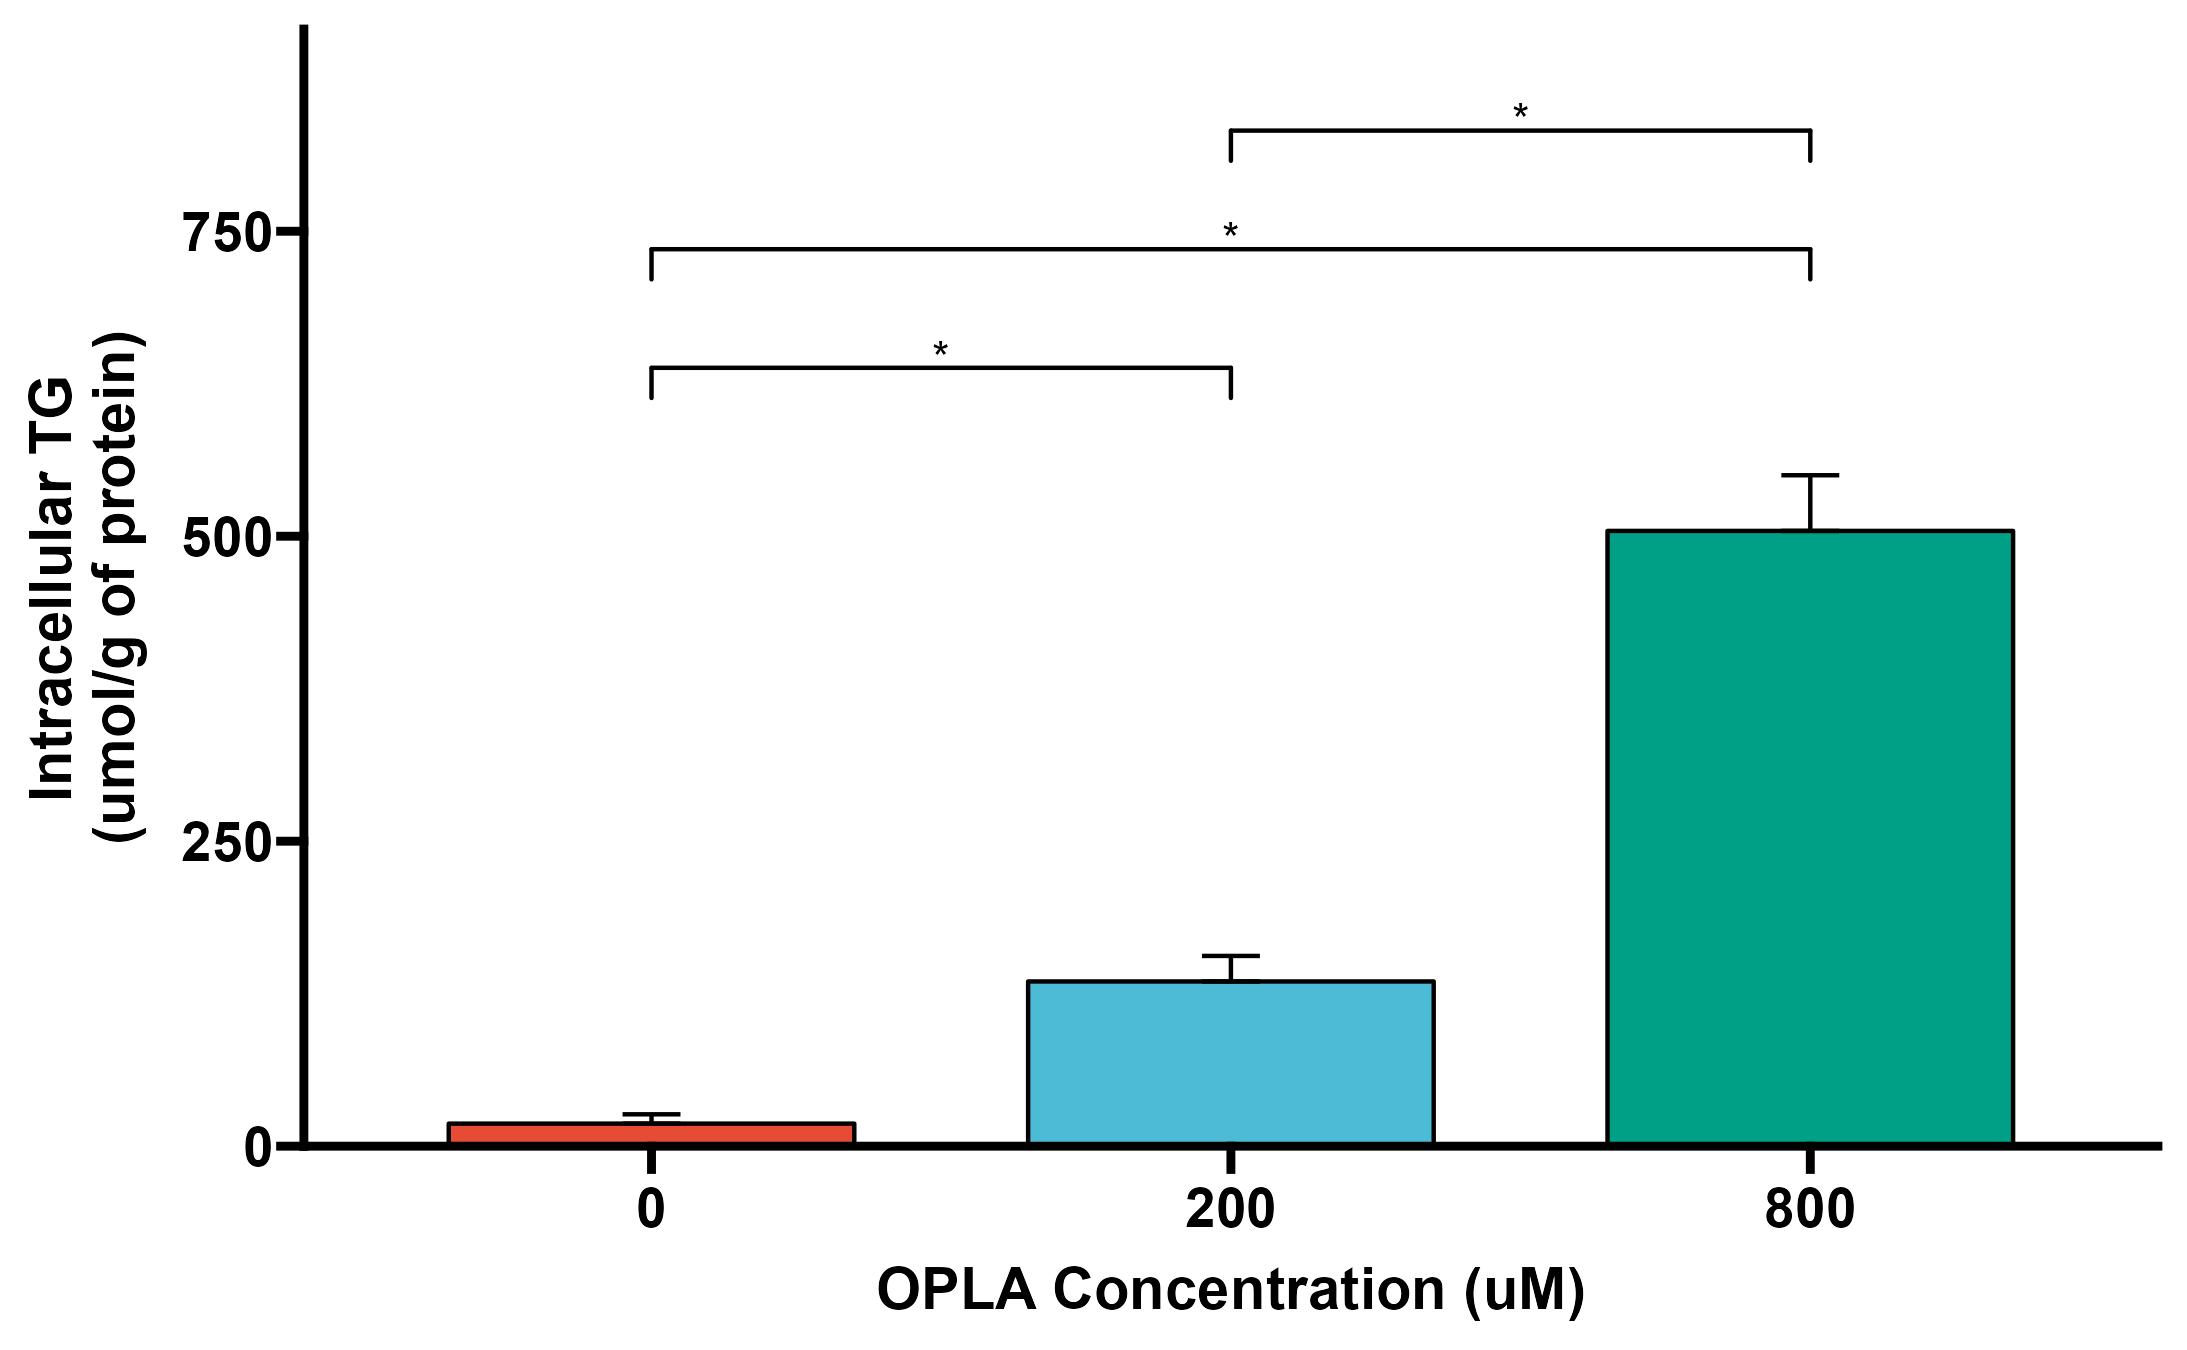
\includegraphics[width=0.49\textwidth]{figures/ch3-Model Development/LFHF TG.png}};
  \tikz\node[inner sep=0pt,label={[anchor=north west]north west:\subref{fig:LFHF ATG genes}}] {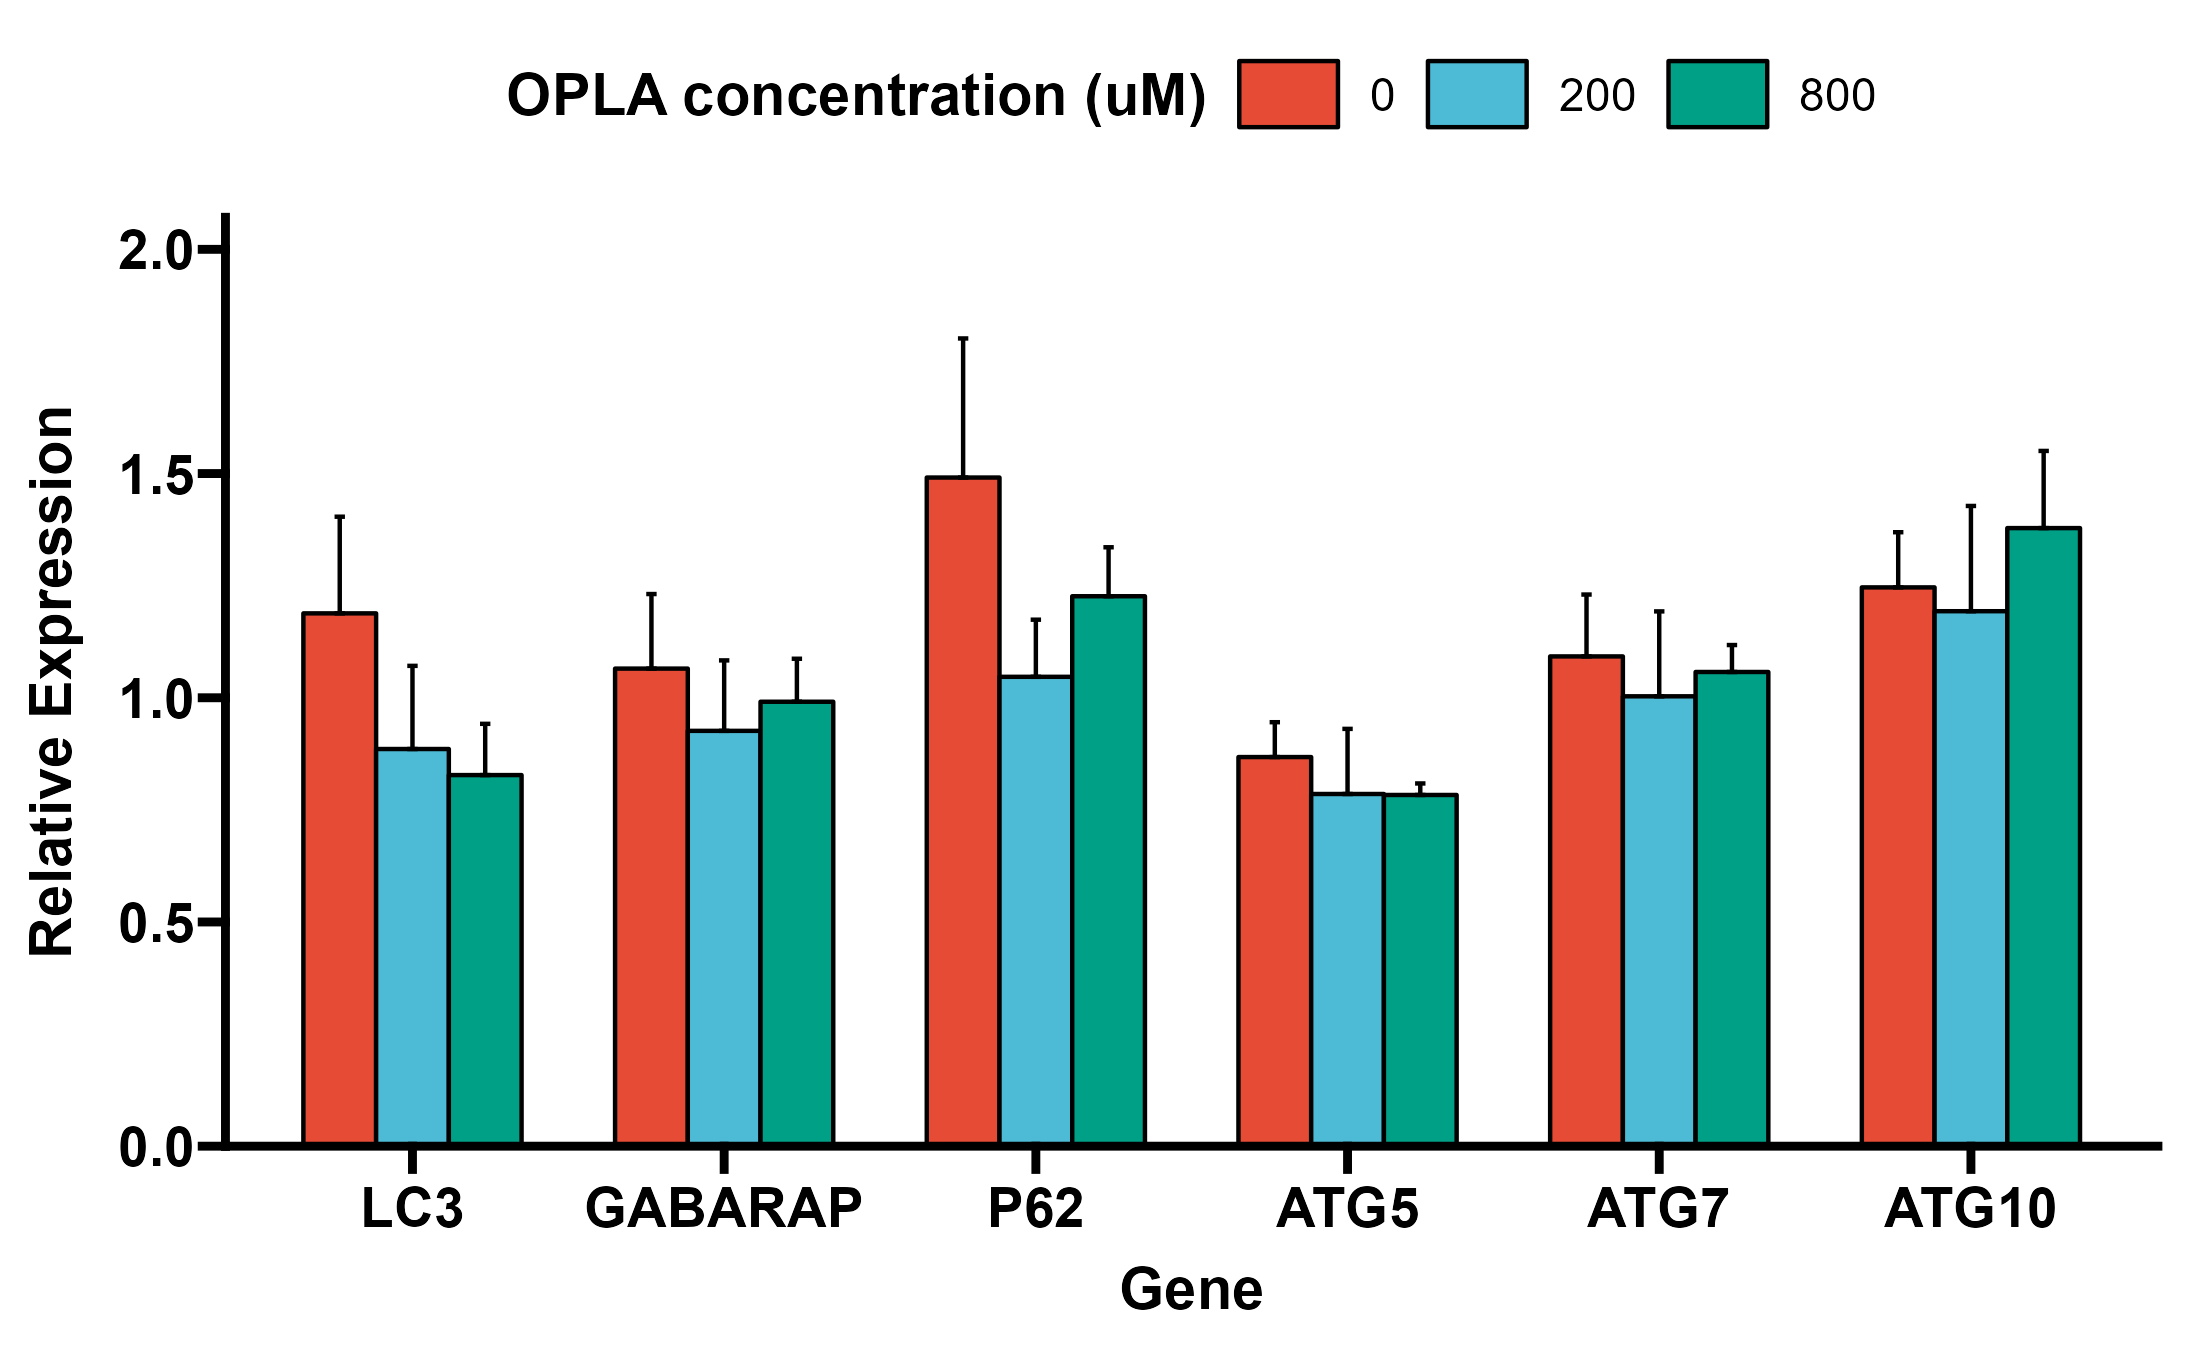
\includegraphics[width=0.49\textwidth]{figures/ch3-Model Development/LFHF ATG genes.png}};
   \tikz\node[inner sep=0pt,label={[anchor=north west]north west:\subref{fig:OPLA 0uM Picture}}] {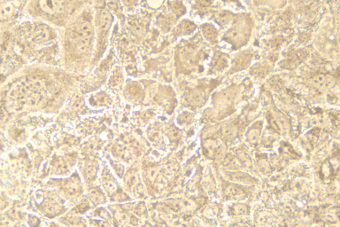
\includegraphics[width=0.49\textwidth]{figures/ch3-Model Development/OPLA 0uM Picture.png}};
      \tikz\node[inner sep=0pt,label={[anchor=north west]north west:\subref{fig:OPLA 800uM Picture}}] {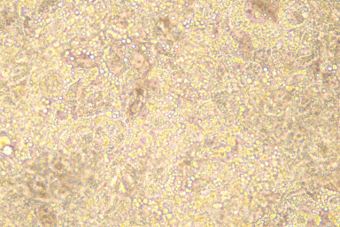
\includegraphics[width=0.49\textwidth]{figures/ch3-Model Development/OPLA 800uM Picture.png}};
    \caption{\textbf{Effect of media FA concentration on TG accumulation and autophagy.} Huh7 cells were cultured for 7 days in increasing concentrations of OPLA fatty acid mix. \textbf{A)} Lipids were extracted and intracellular TG content quantified by gas chromatography. \textbf{B)} RNA was extracted to measure autophagic gene expression relative to three housekeeper genes. Representative images (40x magnification) of cells cultured with \textbf{C)} no FA and in \textbf{D)} 800μM OPLA FA mix. Graphs representative of three biological repeats (n=3) carried out in technical triplicate. * p < 0.05. Abbreviations: TG, Triglyceride.}
            \label{fig:ch3-Model Development LFHF}
\end{figure}


\subsection{Effect of media FA composition on TG accumulation and autophagy}

Culturing Huh7 cells in predominantly unsaturated (OPLA) or saturated (POLA) FAs resulted in a similar increase in intracellular TG content, when compared to control media free from FAs (Figure \ref{fig:OPLAPOLA TG}). Intracellular TG composition reflected that of the FAs the cells were cultured in (Figure \ref{fig:OPLAPOLA Lipid}). Autophagic flux was then assessed by measuring LC3-II protein intensity (relative to housekeeper protein $\alpha$-Tubulin) with and without the autophagic inhibitor BAF. As LC3-II is normally degraded during autophagy, it's accumulation during autophagic inhibition is reflective of overall autophagic flux \cite{DJ2021Guidelines1}. There was no significant difference in autophagic flux between control, OPLA and POLA conditions, though there was a trend towards a decrease in cells treated with FAs (Figures \ref{fig:OPLAPOLA ATG FLX} - \ref{fig:OPLAPOLA WB Photo}).

\begin{figure}[h!]
  \centering
  {\phantomsubcaption\label{fig:OPLAPOLA TG}}
  {\phantomsubcaption\label{fig:OPLAPOLA Lipid}}
   {\phantomsubcaption\label{fig:OPLAPOLA ATG FLX}}
    {\phantomsubcaption\label{fig:OPLAPOLA BAF}}
     {\phantomsubcaption\label{fig:OPLAPOLA WB Photo}}
  \tikz\node[inner sep=0pt,label={[anchor=north west]north west:\subref{fig:OPLAPOLA TG}}] {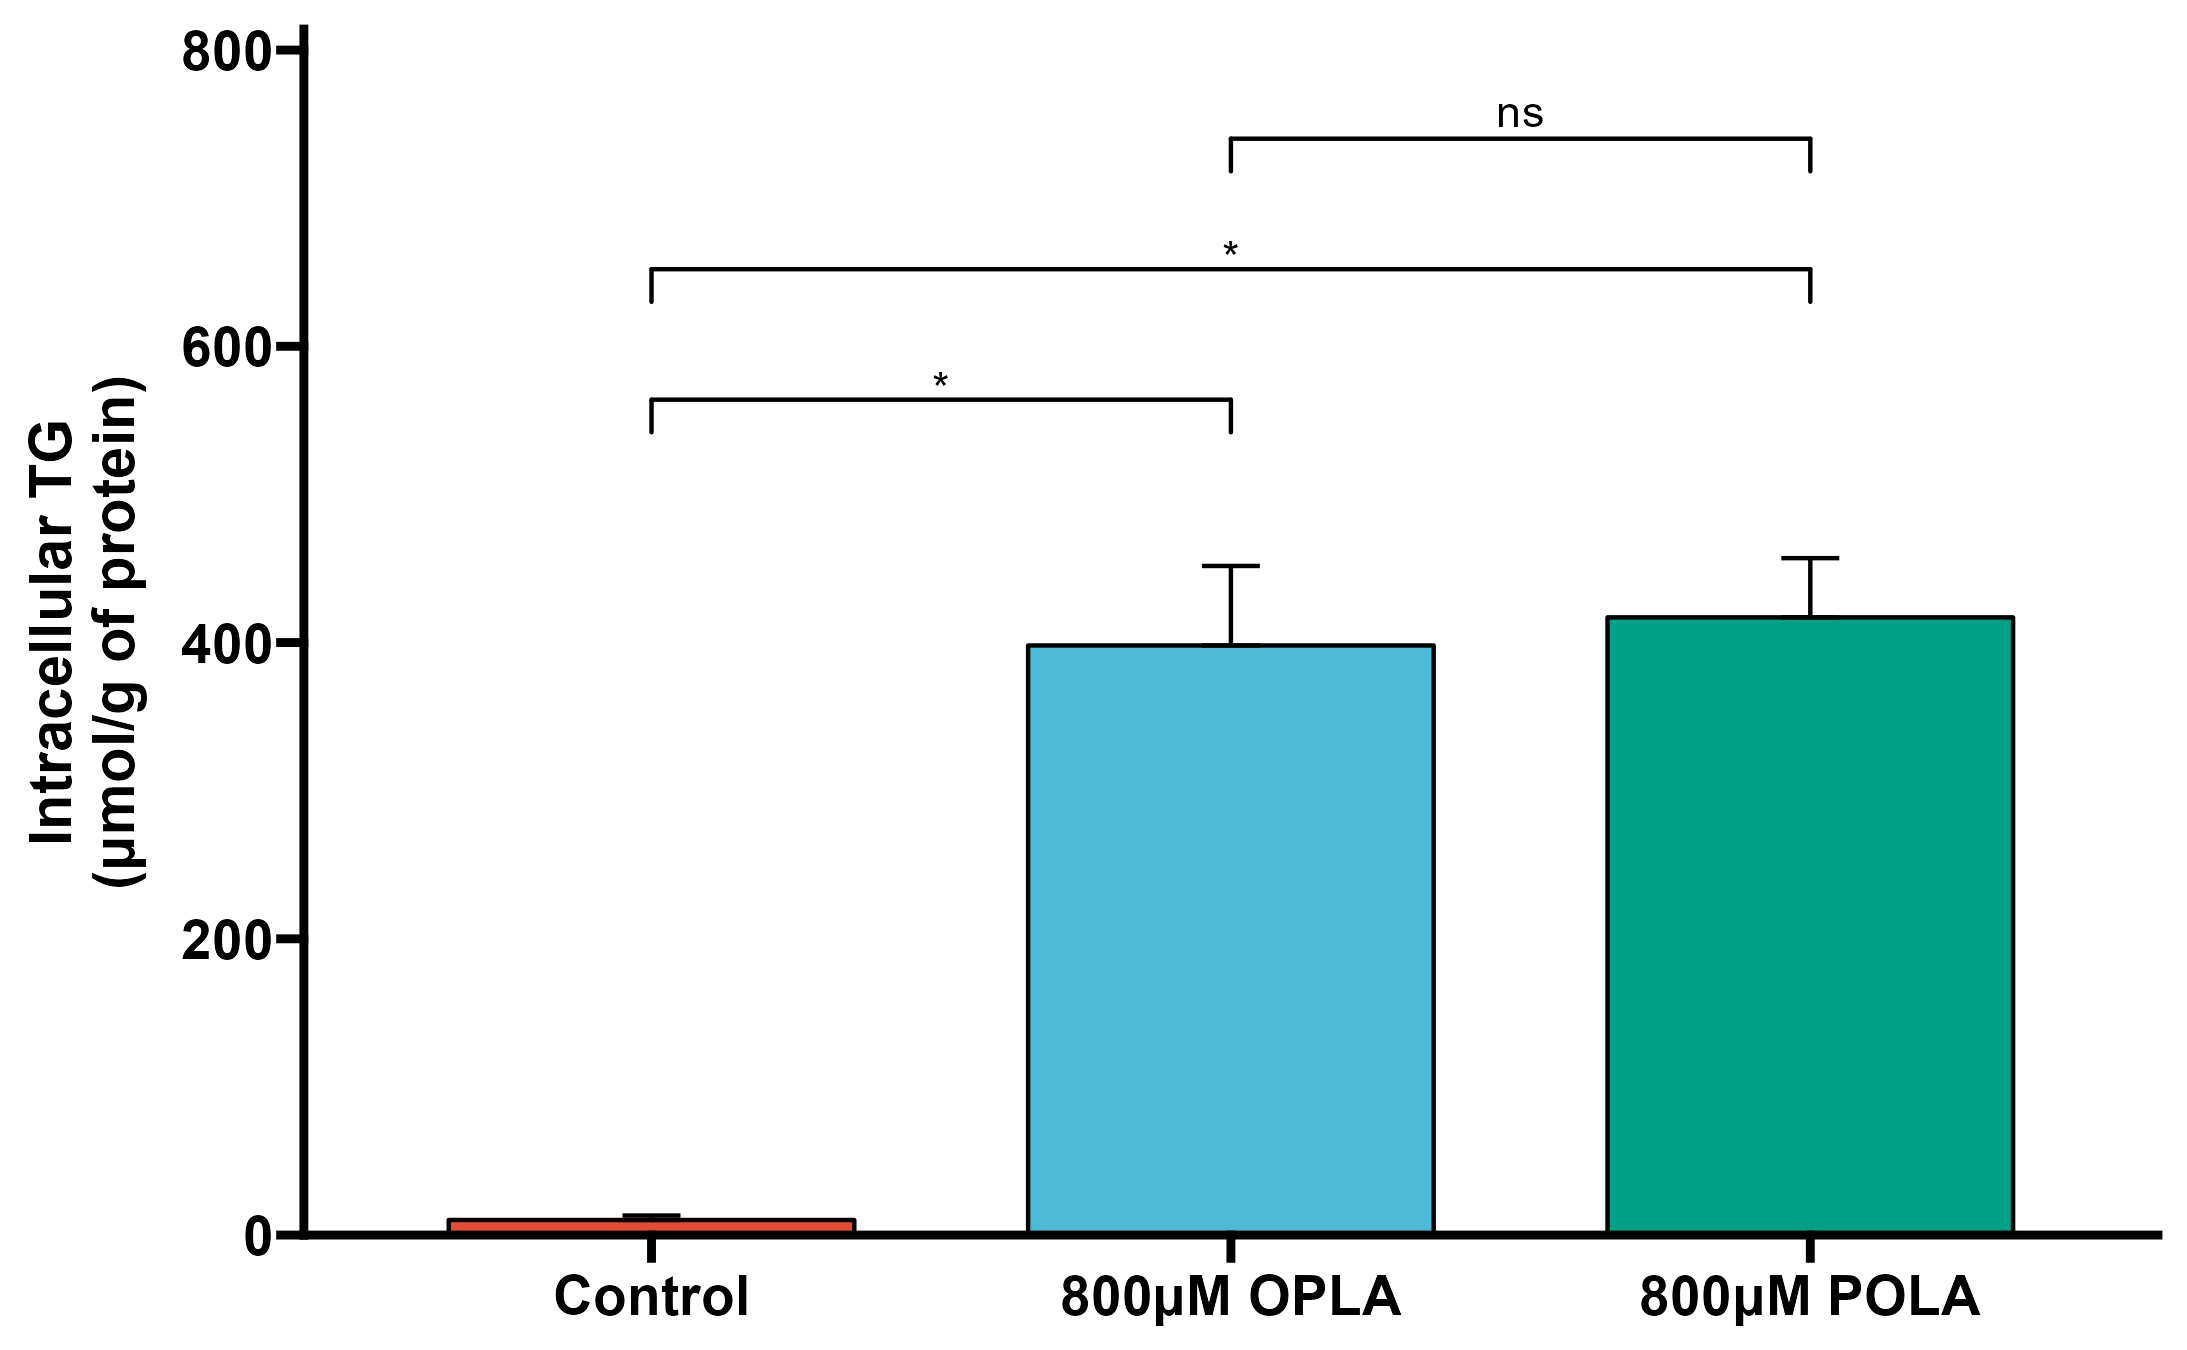
\includegraphics[width=0.49\textwidth]{figures/ch3-Model Development/OPLAPOLA TG.png}};
  \tikz\node[inner sep=0pt,label={[anchor=north west]north west:\subref{fig:OPLAPOLA Lipid}}] {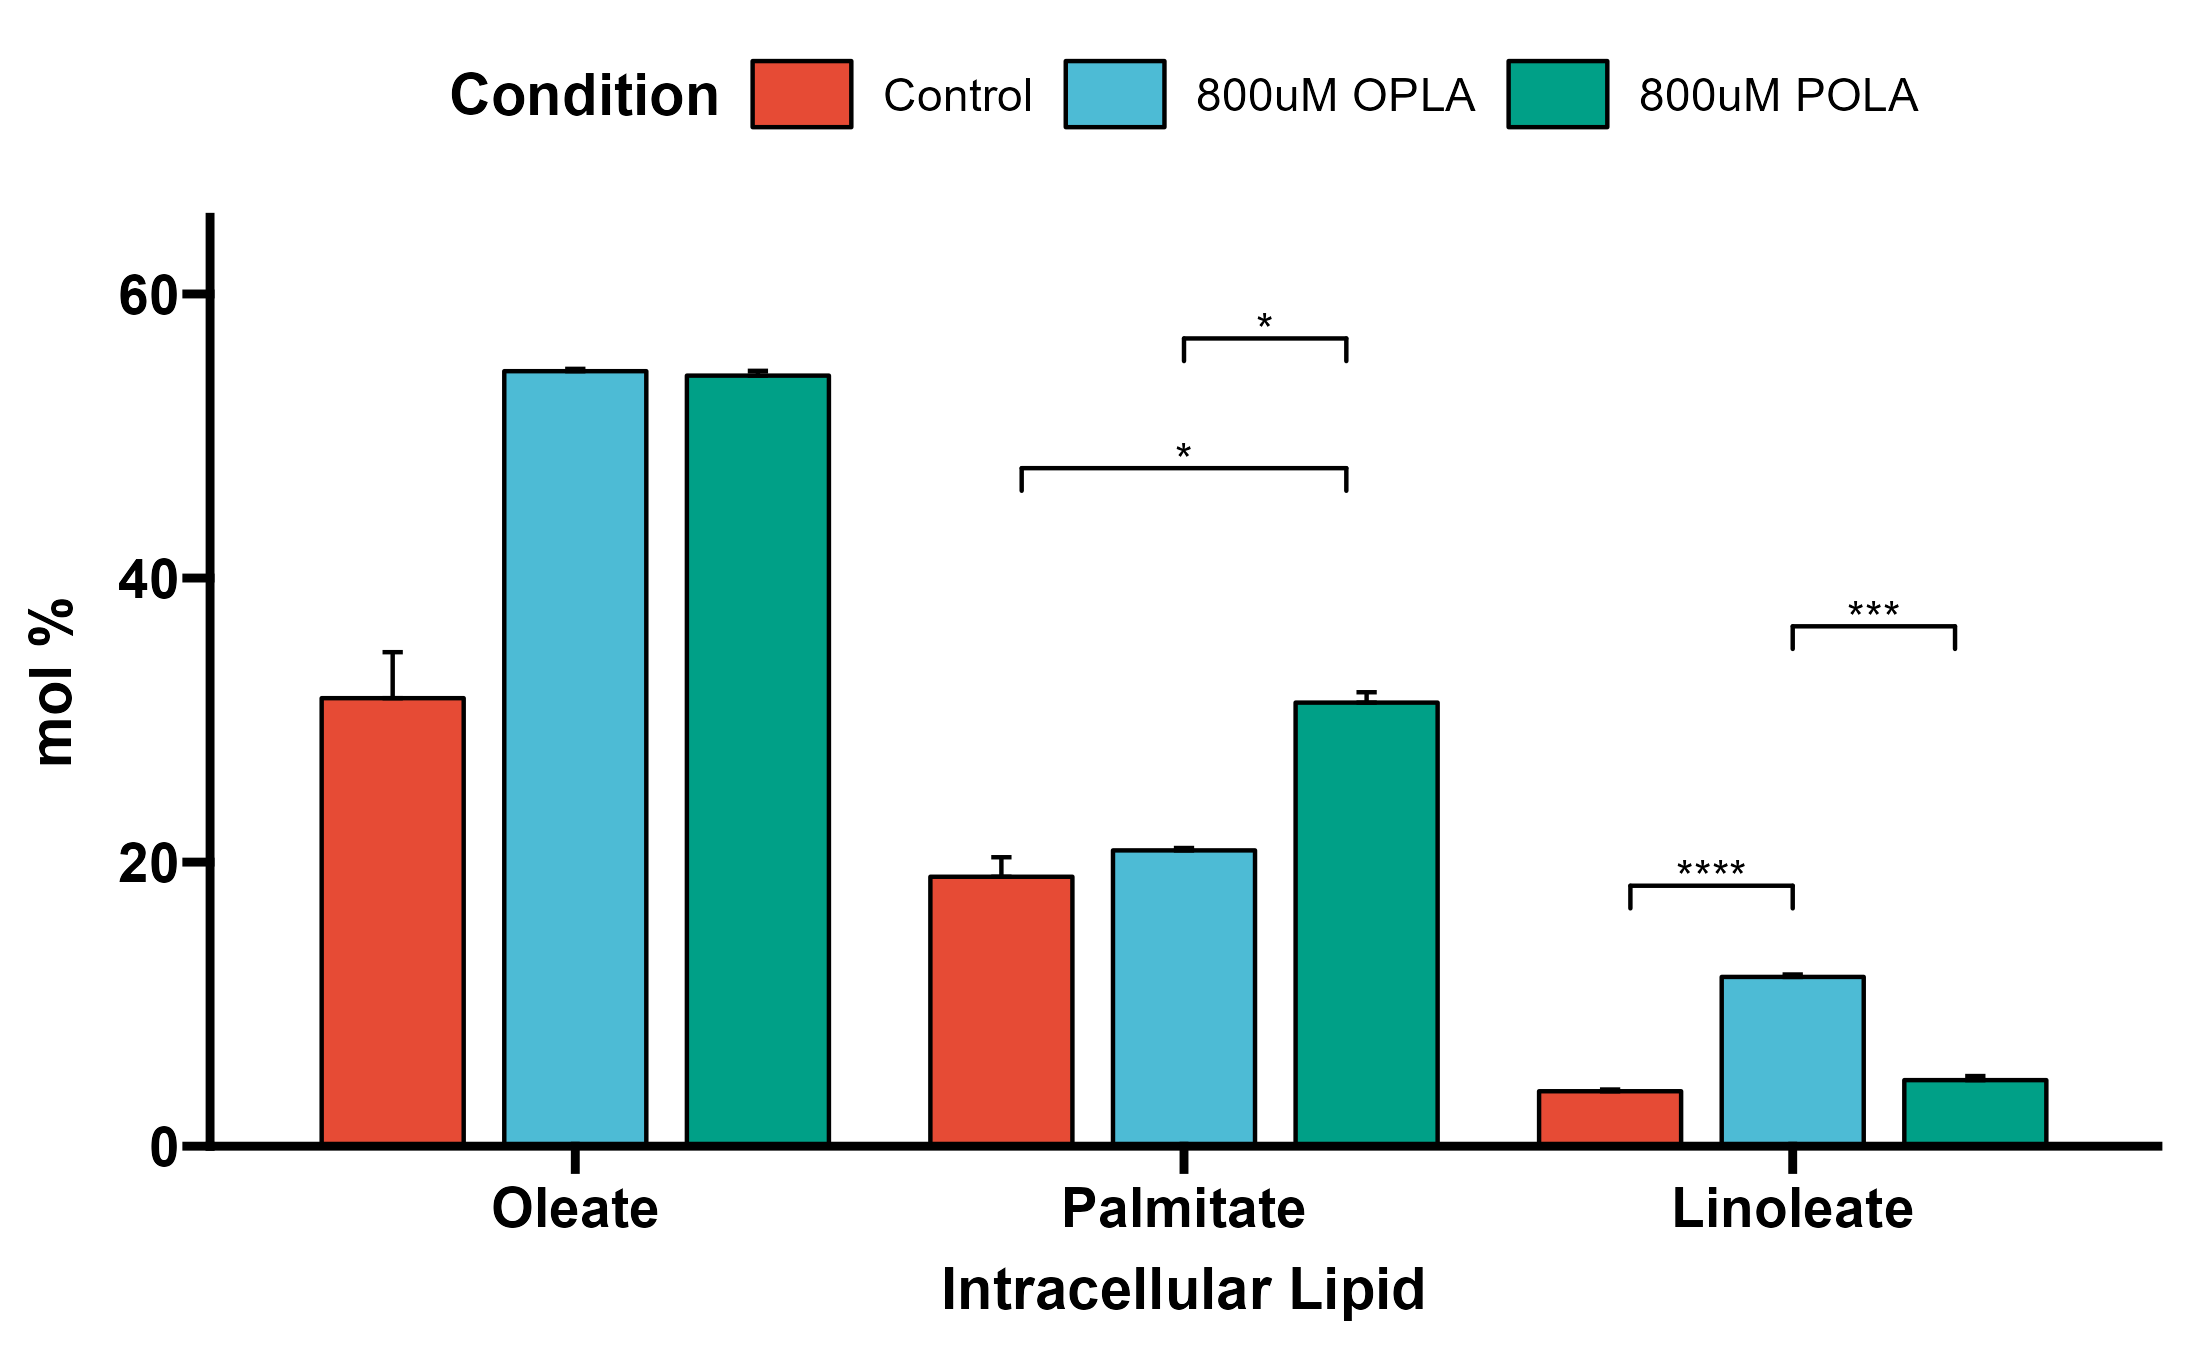
\includegraphics[width=0.49\textwidth]{figures/ch3-Model Development/OPLAPOLA Lipid contributions.png}};
   \tikz\node[inner sep=0pt,label={[anchor=north west]north west:\subref{fig:OPLAPOLA ATG FLX}}] {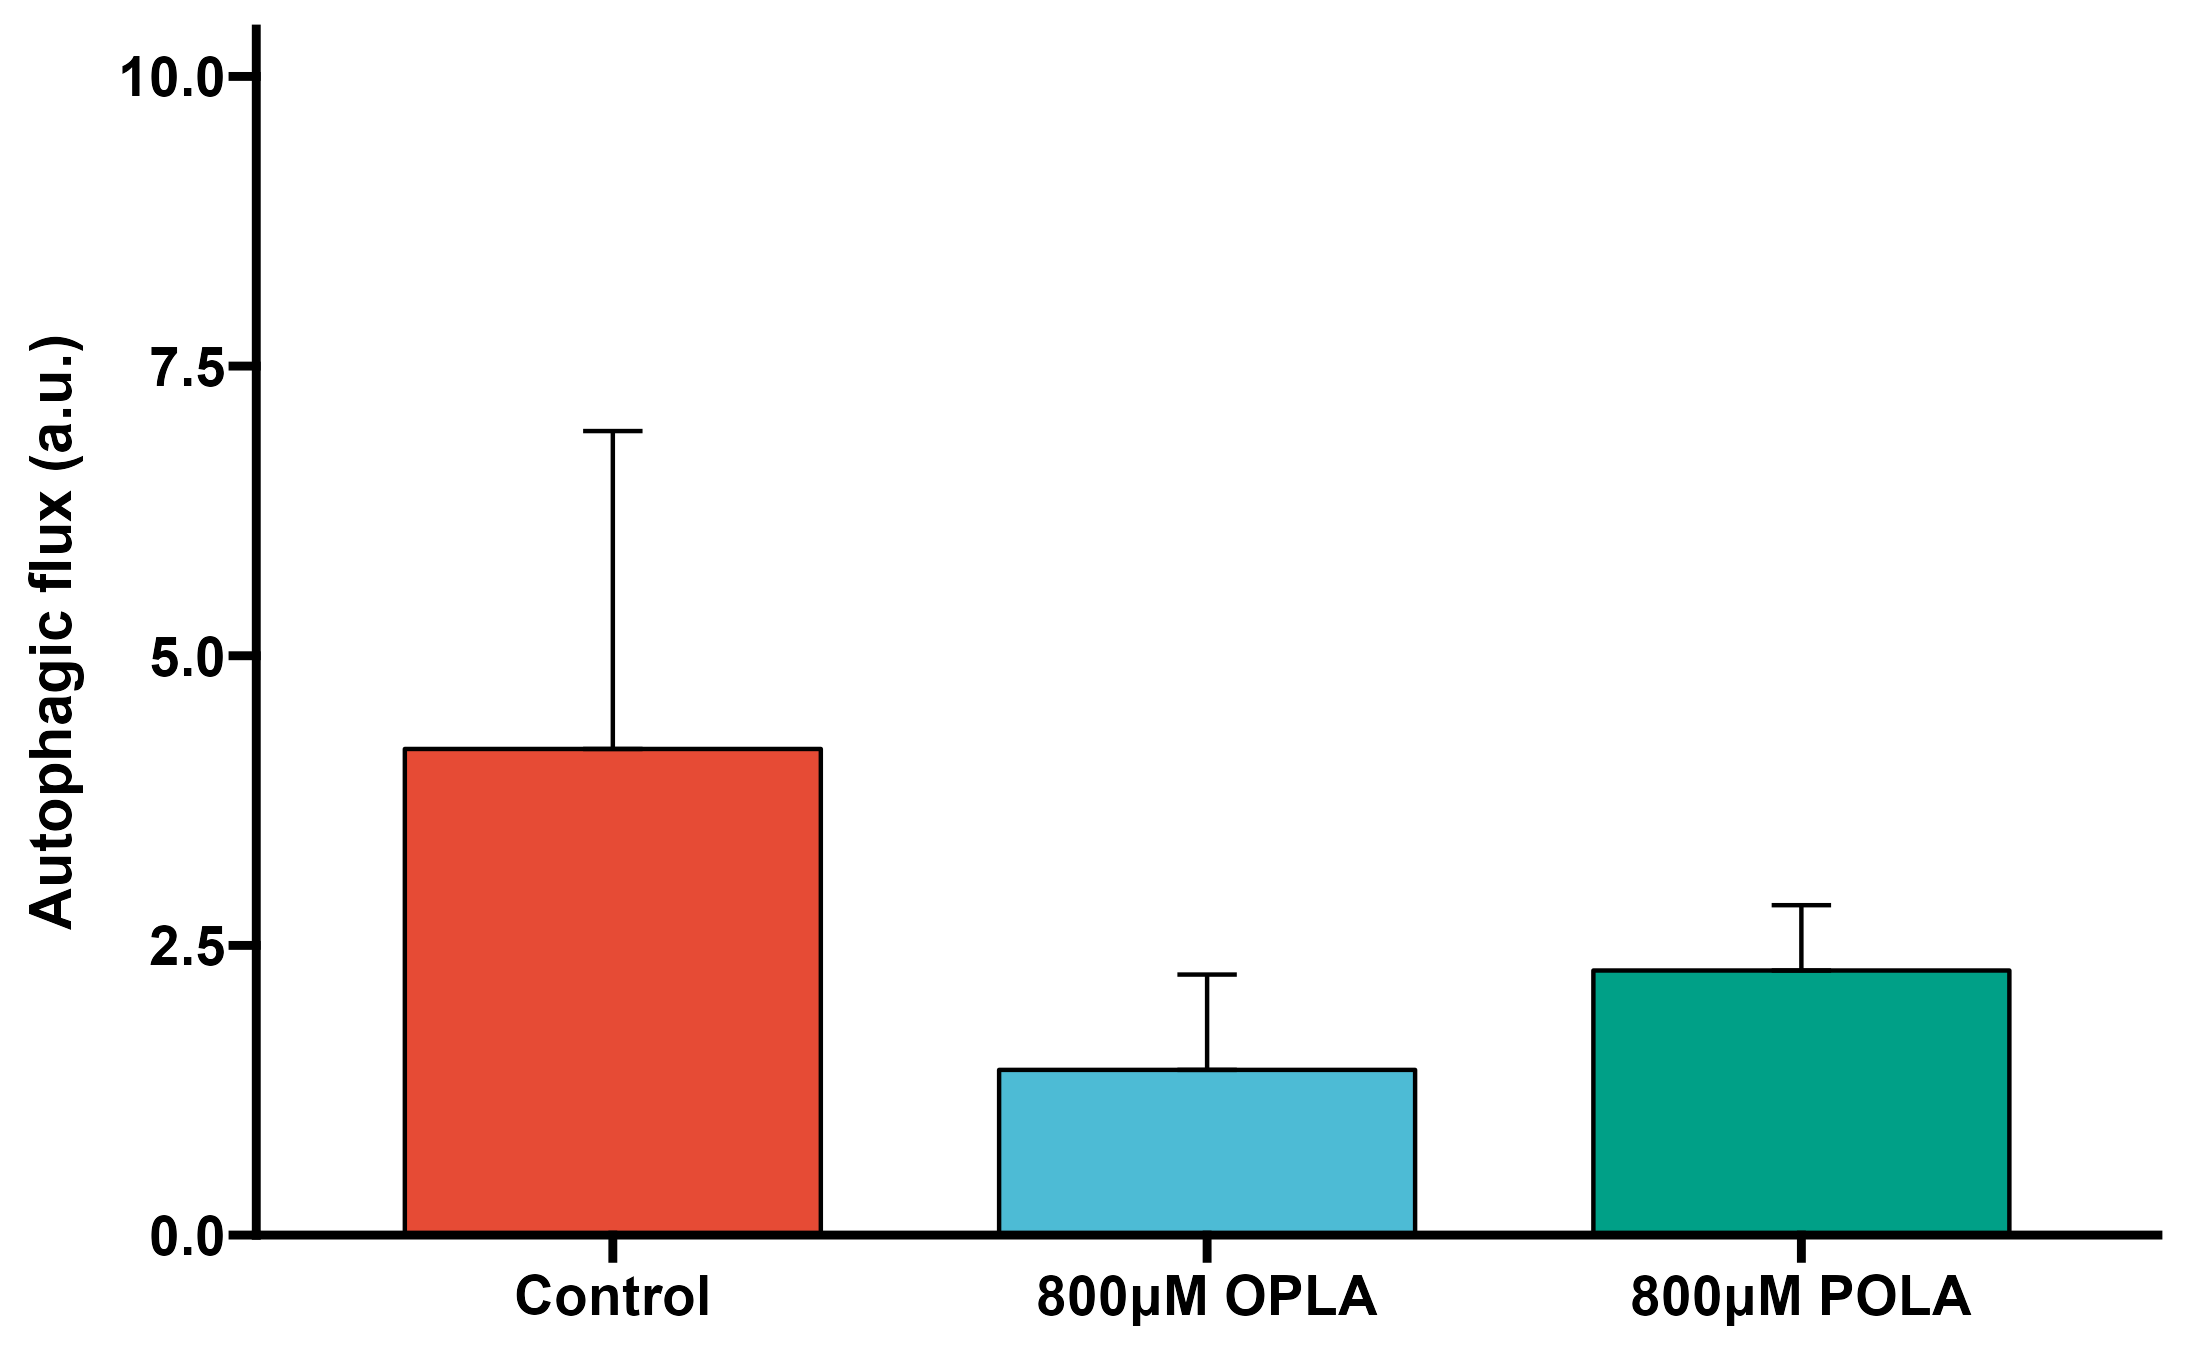
\includegraphics[width=0.49\textwidth]{figures/ch3-Model Development/OPLAPOLA ATG FLX.png}};
      \tikz\node[inner sep=0pt,label={[anchor=north west]north west:\subref{fig:OPLAPOLA BAF}}] {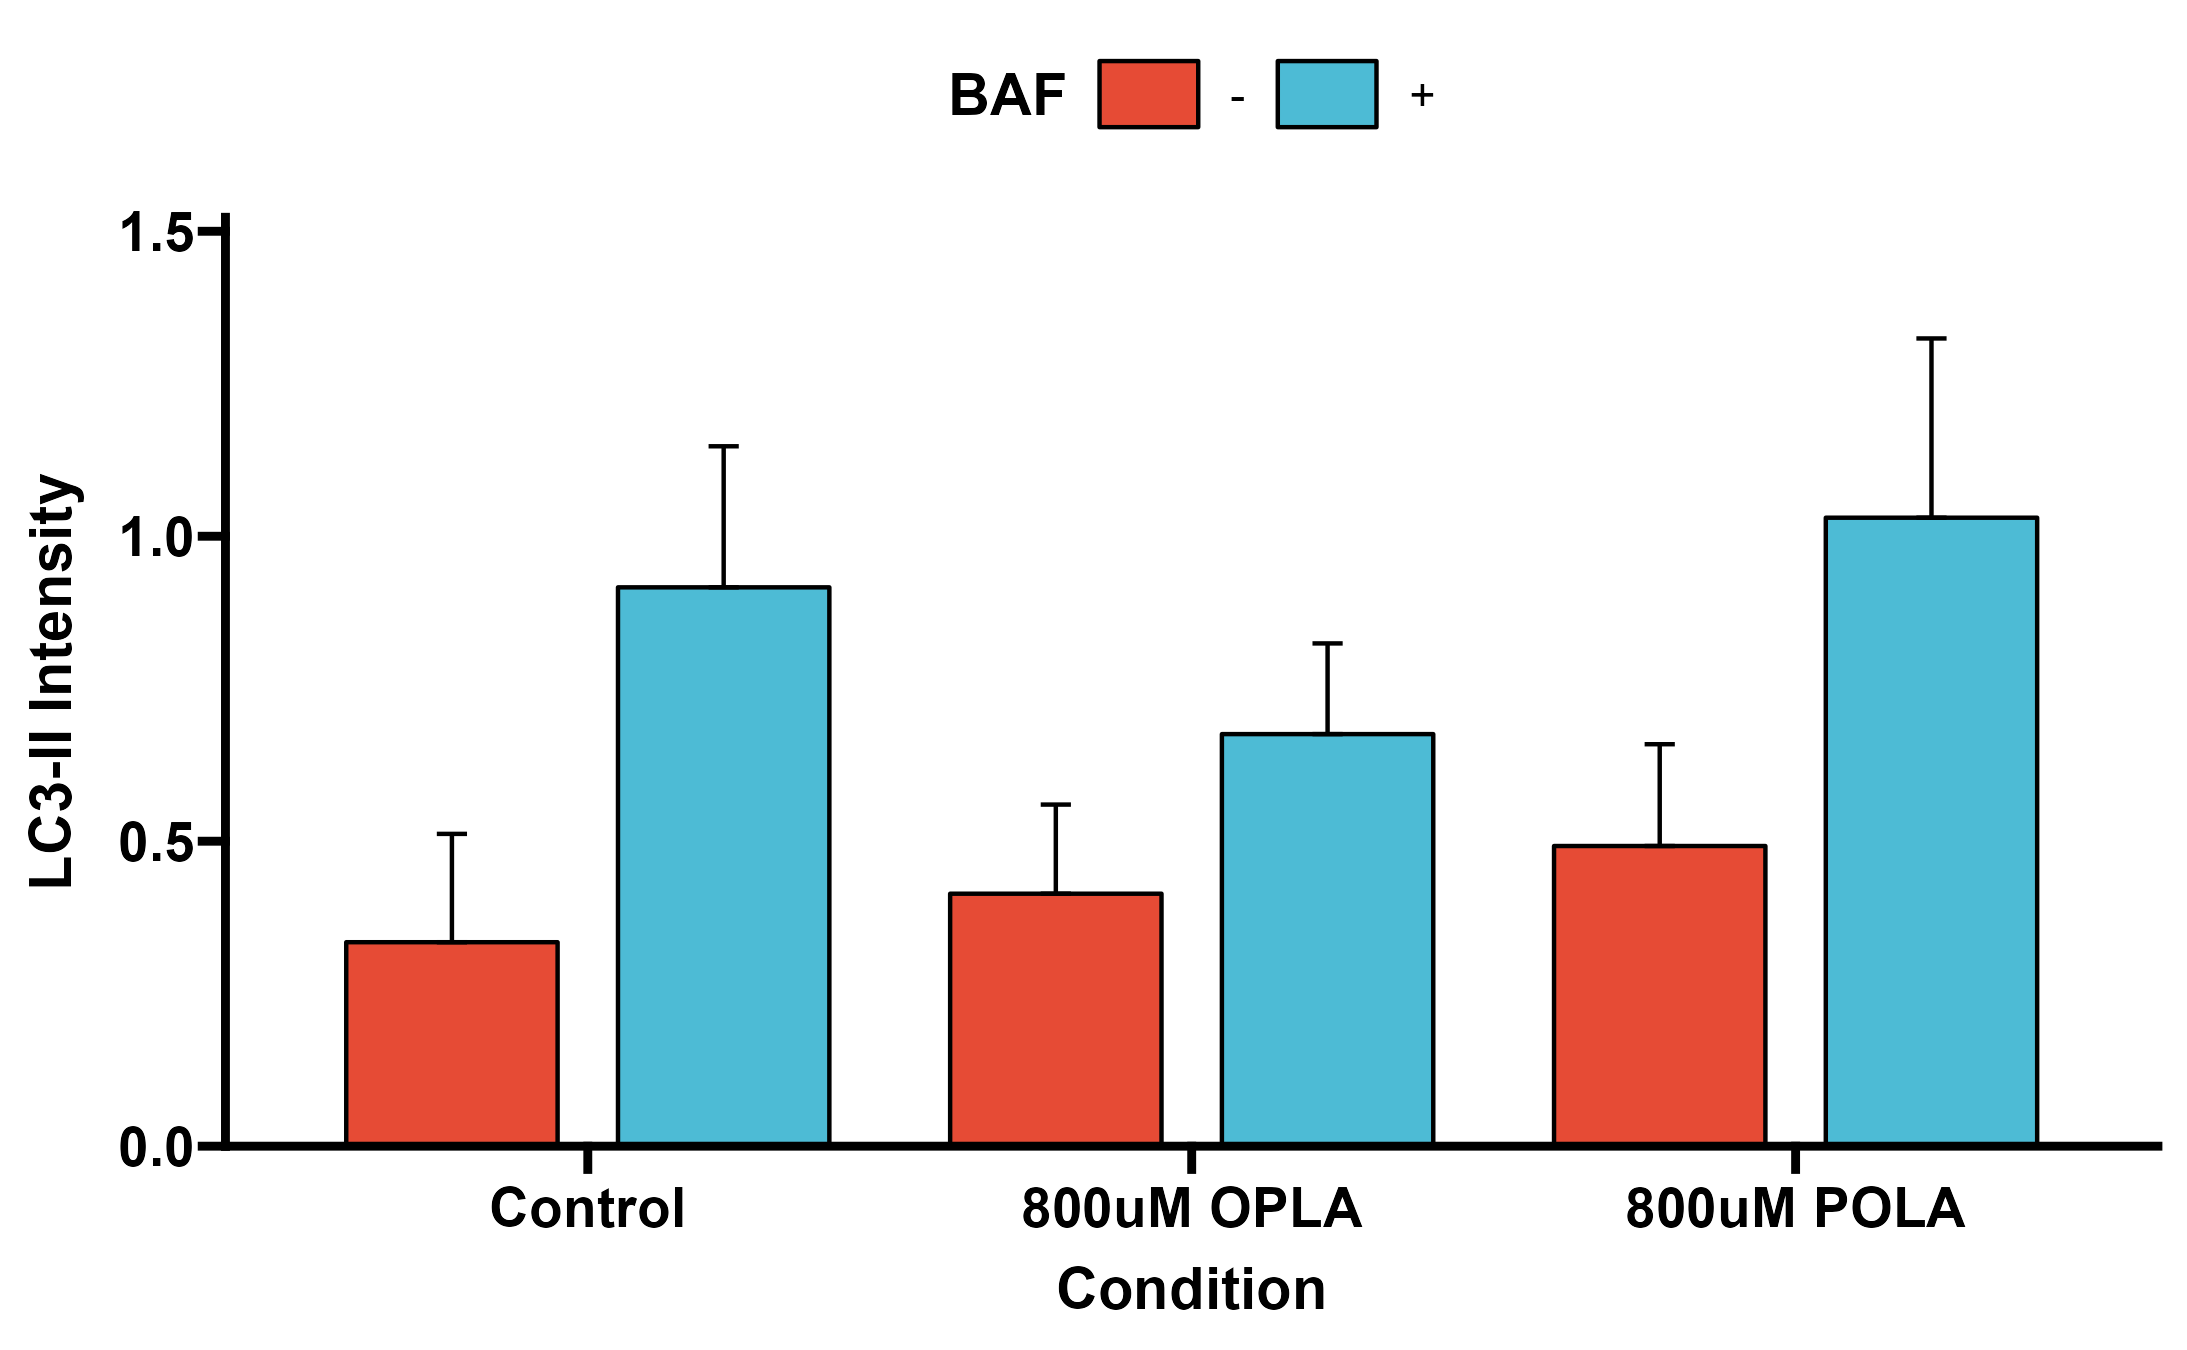
\includegraphics[width=0.49\textwidth]{figures/ch3-Model Development/OPLAPOLA BAF.png}};
      \tikz\node[inner sep=0pt,label={[anchor=north west]north west:\subref{fig:OPLAPOLA WB Photo}}] {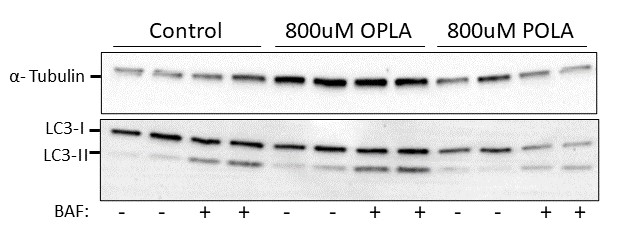
\includegraphics[width=0.6\textwidth]{figures/ch3-Model Development/OPLAPOLA WB Photo.jpg}};
        \caption{\textbf{Effect of media FA composition on TG accumulation and autophagy.} Cells were cultured for 7 days in either media with no FA (Control), a predominantly unsaturated FA mix (OPLA) or a predominantly saturated FA mix (POLA). Lipids were extracted and quantified by gas chromatography to measure \textbf{A)} total intracellular TG and \textbf{B)} the composition of intracellular TG. \textbf{C-E)} Autophagic flux was calculated as LC3-II intensity (relative to housekeeper protein $\alpha$-Tubulin): (BAF - Basal)/Basal. Representative of three biological repeats (n=3) carried out in technical duplicate. * p < 0.05, ** p < 0.01, *** p < 0.001. Abbreviations: BAF, Bafilomycin A1; TG, Triglyceride.}
        \label{fig:OPLAPOLA}
\end{figure}

RNA sequencing data of cells cultured in media supplemented with 800 \uM OPLA or POLA or free from FAs (Control) was analysed to provide further insight. Principle component analysis (PCA) showed that the difference in gene expression between control and OPLA/POLA conditions accounted for the largest component of the total variance (dimension 1 - 77.1\%) and that media FA composition (OPLA vs POLA) accounted for the second largest component (dimension 2 - 9.3\%) as shown in Figure \ref{fig:PCA}. A heatmap representing differential expression of genes involved in autophagic activation \cite{Bordi2021ATranscription} confirmed an overall suppression of autophagic processes in OPLA- and POLA-treated cells compared to controls cells (Figure \ref{fig:ATG heatmap}). Gene set enrichment analysis (GSEA) showed that DNA replication and cell cycle associated genes were the most significantly activated pathways whereas autophagy, infection and endoplasmic reticulum protein processing pathways were most significantly suppressed pathways in both OPLA and POLA treated cells compared to control cells (Figures \ref{fig:OPLA GSEA} and \ref{fig:POLA GSEA}).

\begin{figure}[h!]
  \centering
  {\phantomsubcaption\label{fig:PCA}}
  {\phantomsubcaption\label{fig:ATG heatmap}}
   {\phantomsubcaption\label{fig:OPLA GSEA}}
    {\phantomsubcaption\label{fig:POLA GSEA}}
  \tikz\node[inner sep=0pt,label={[anchor=north west]north west:\subref{fig:PCA}}] {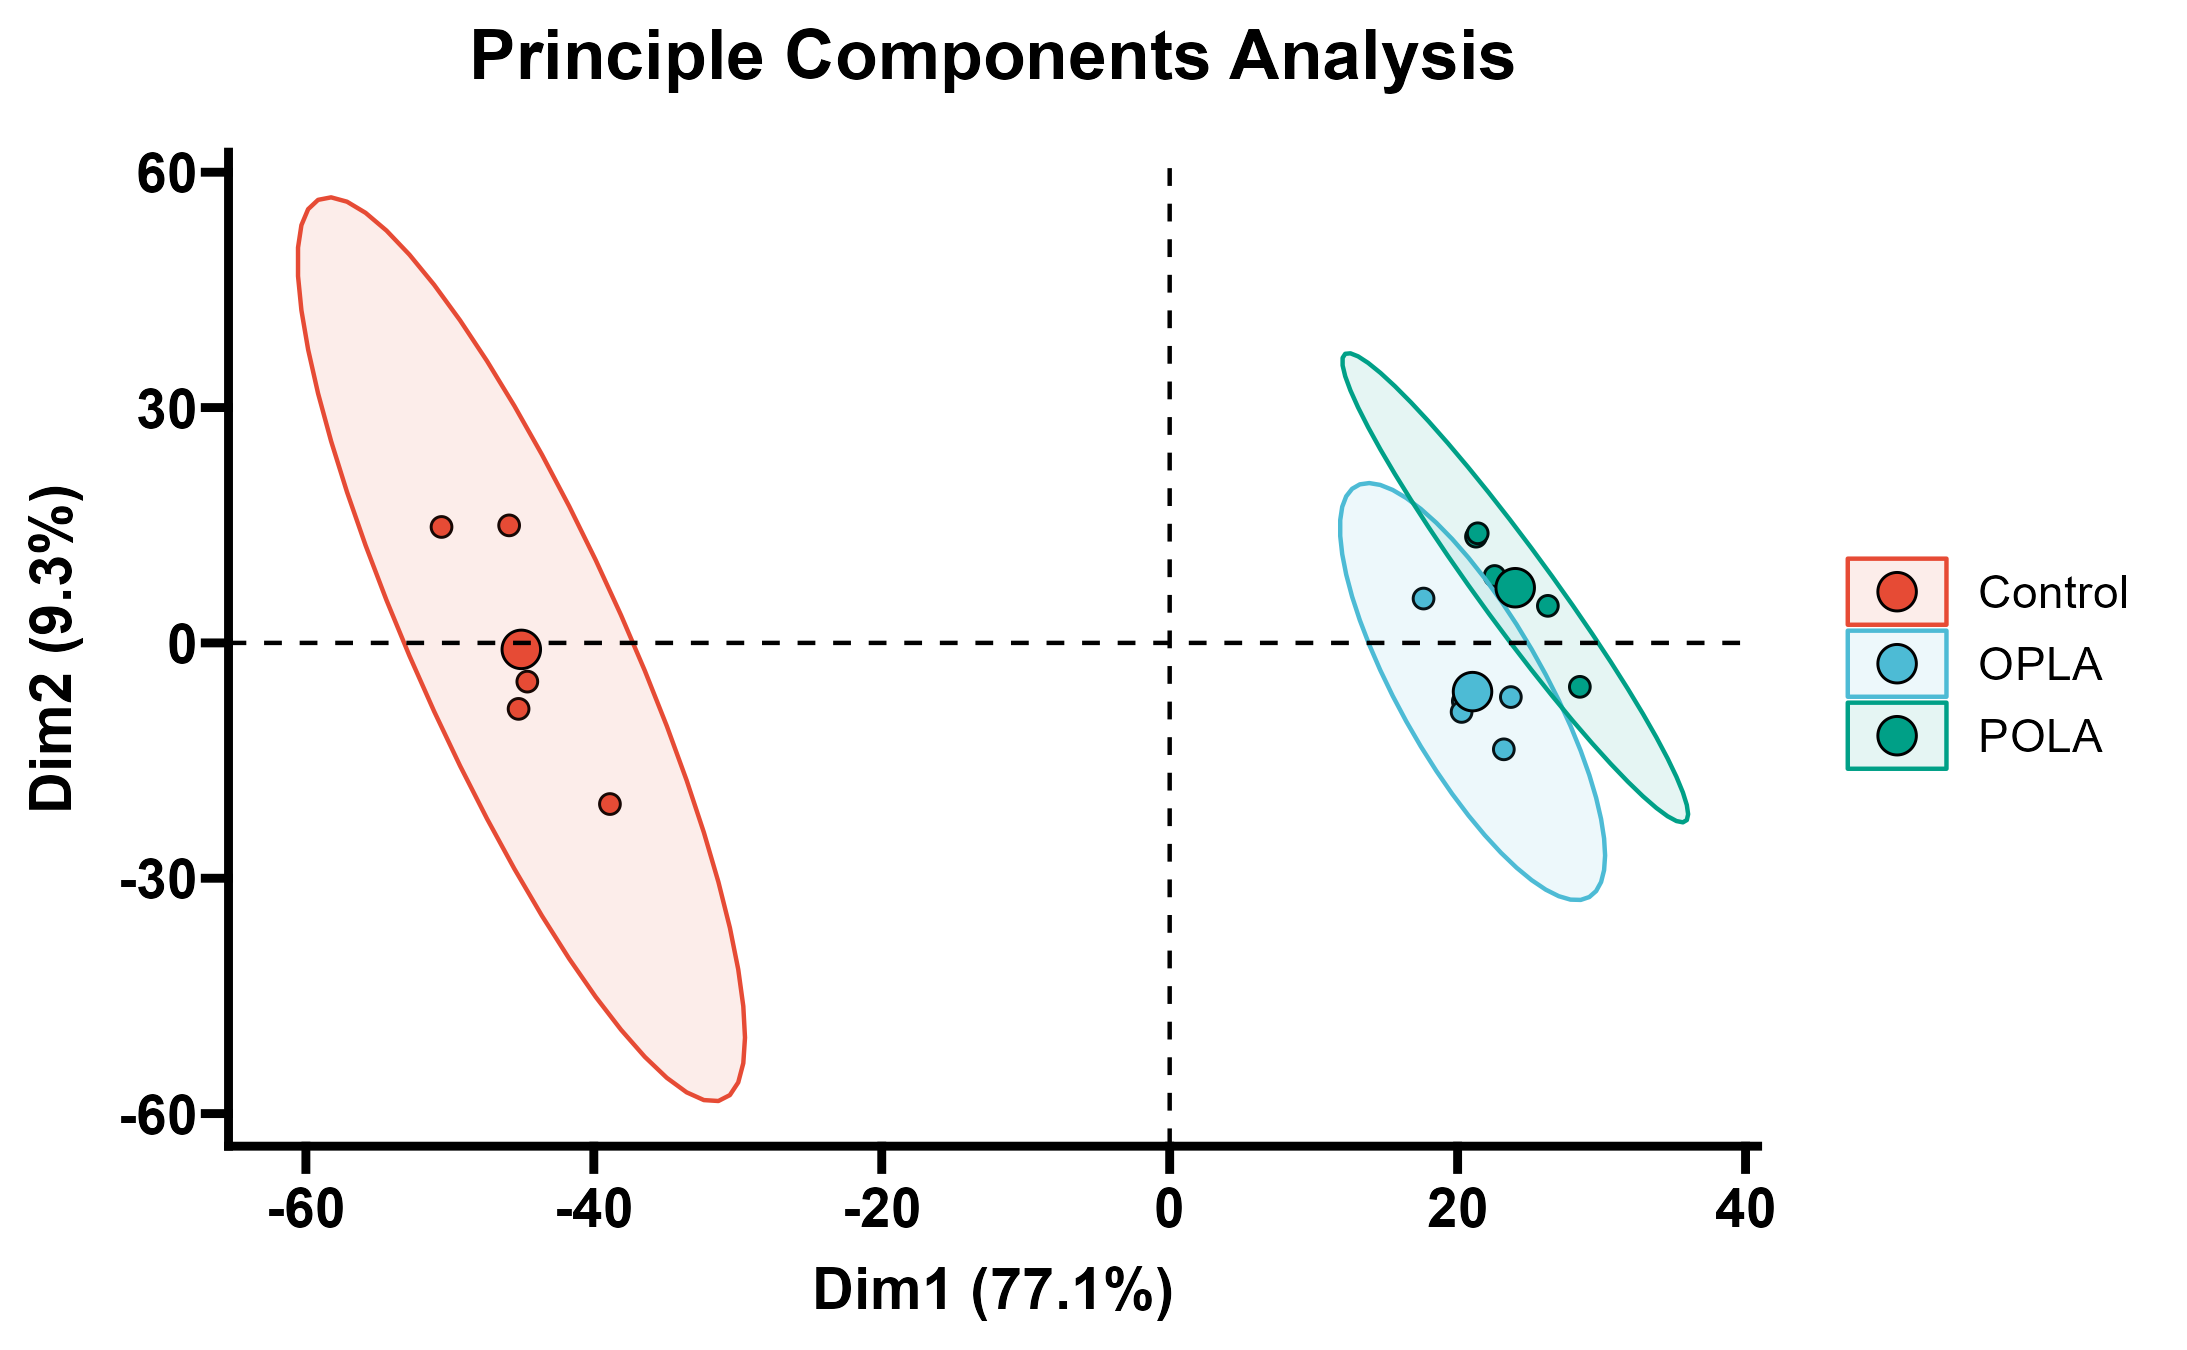
\includegraphics[width=0.49\textwidth]{figures/ch3-Model Development/PCA.png}};
  \tikz\node[inner sep=0pt,label={[anchor=north west]north west:\subref{fig:ATG heatmap}}] {
\includegraphics[width=0.49\textwidth]{figures/ch3-Model Development/ATG heatmap.png}};
   \tikz\node[inner sep=0pt,label={[anchor=north west]north west:\subref{fig:OPLA GSEA}}] {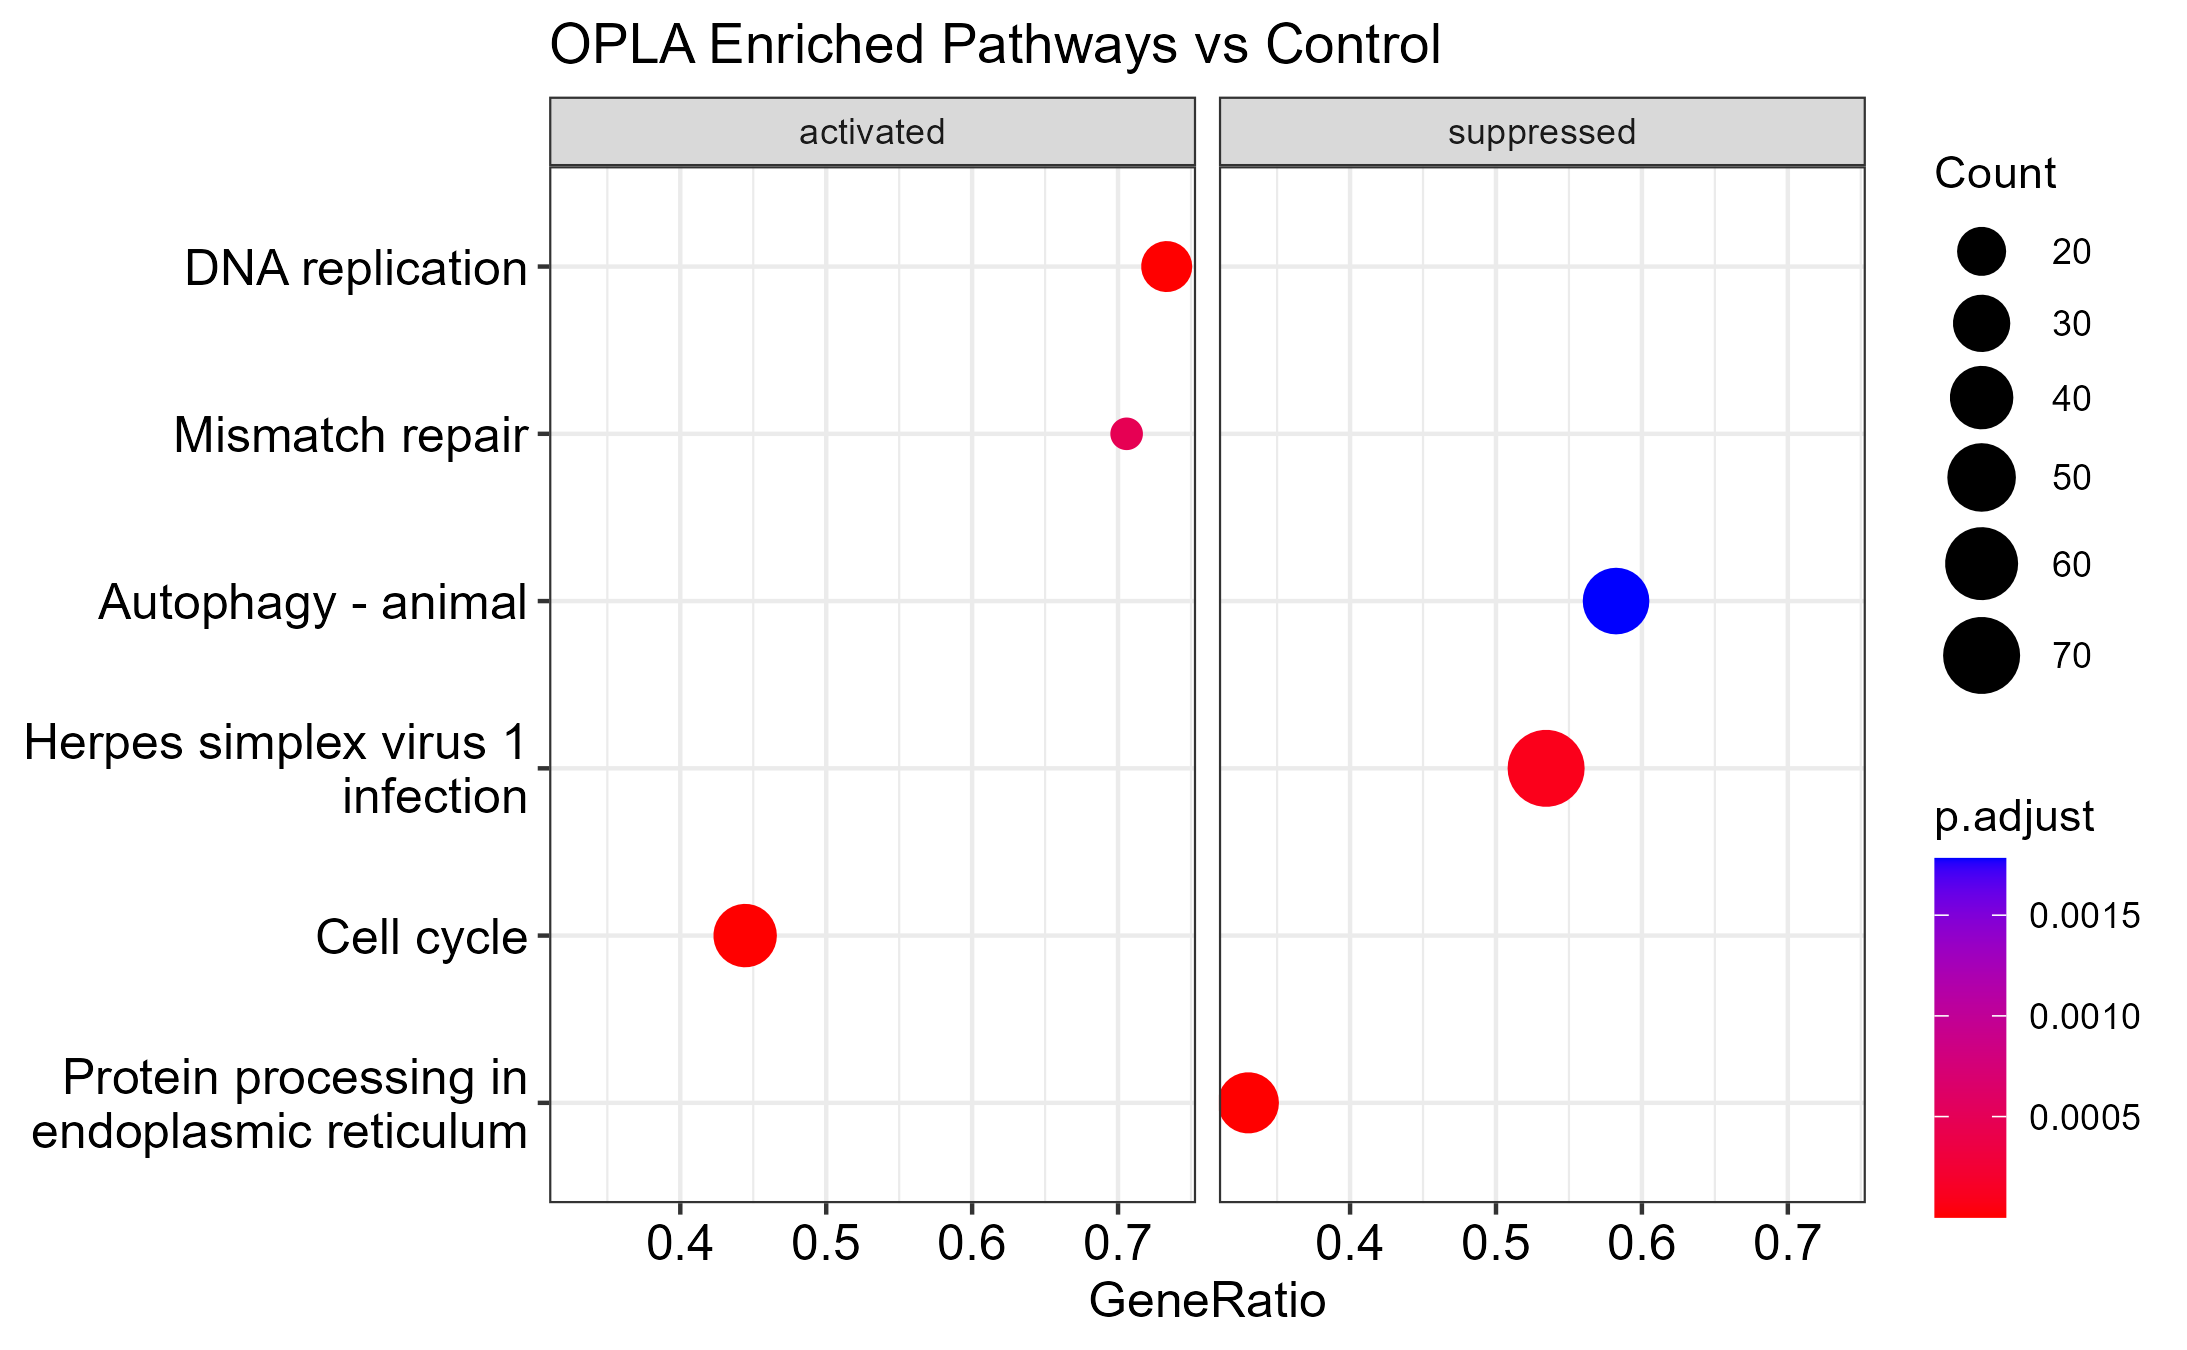
\includegraphics[width=0.49\textwidth]{figures/ch3-Model Development/OPLA GSEA.png}};
      \tikz\node[inner sep=0pt,label={[anchor=north west]north west:\subref{fig:POLA GSEA}}] {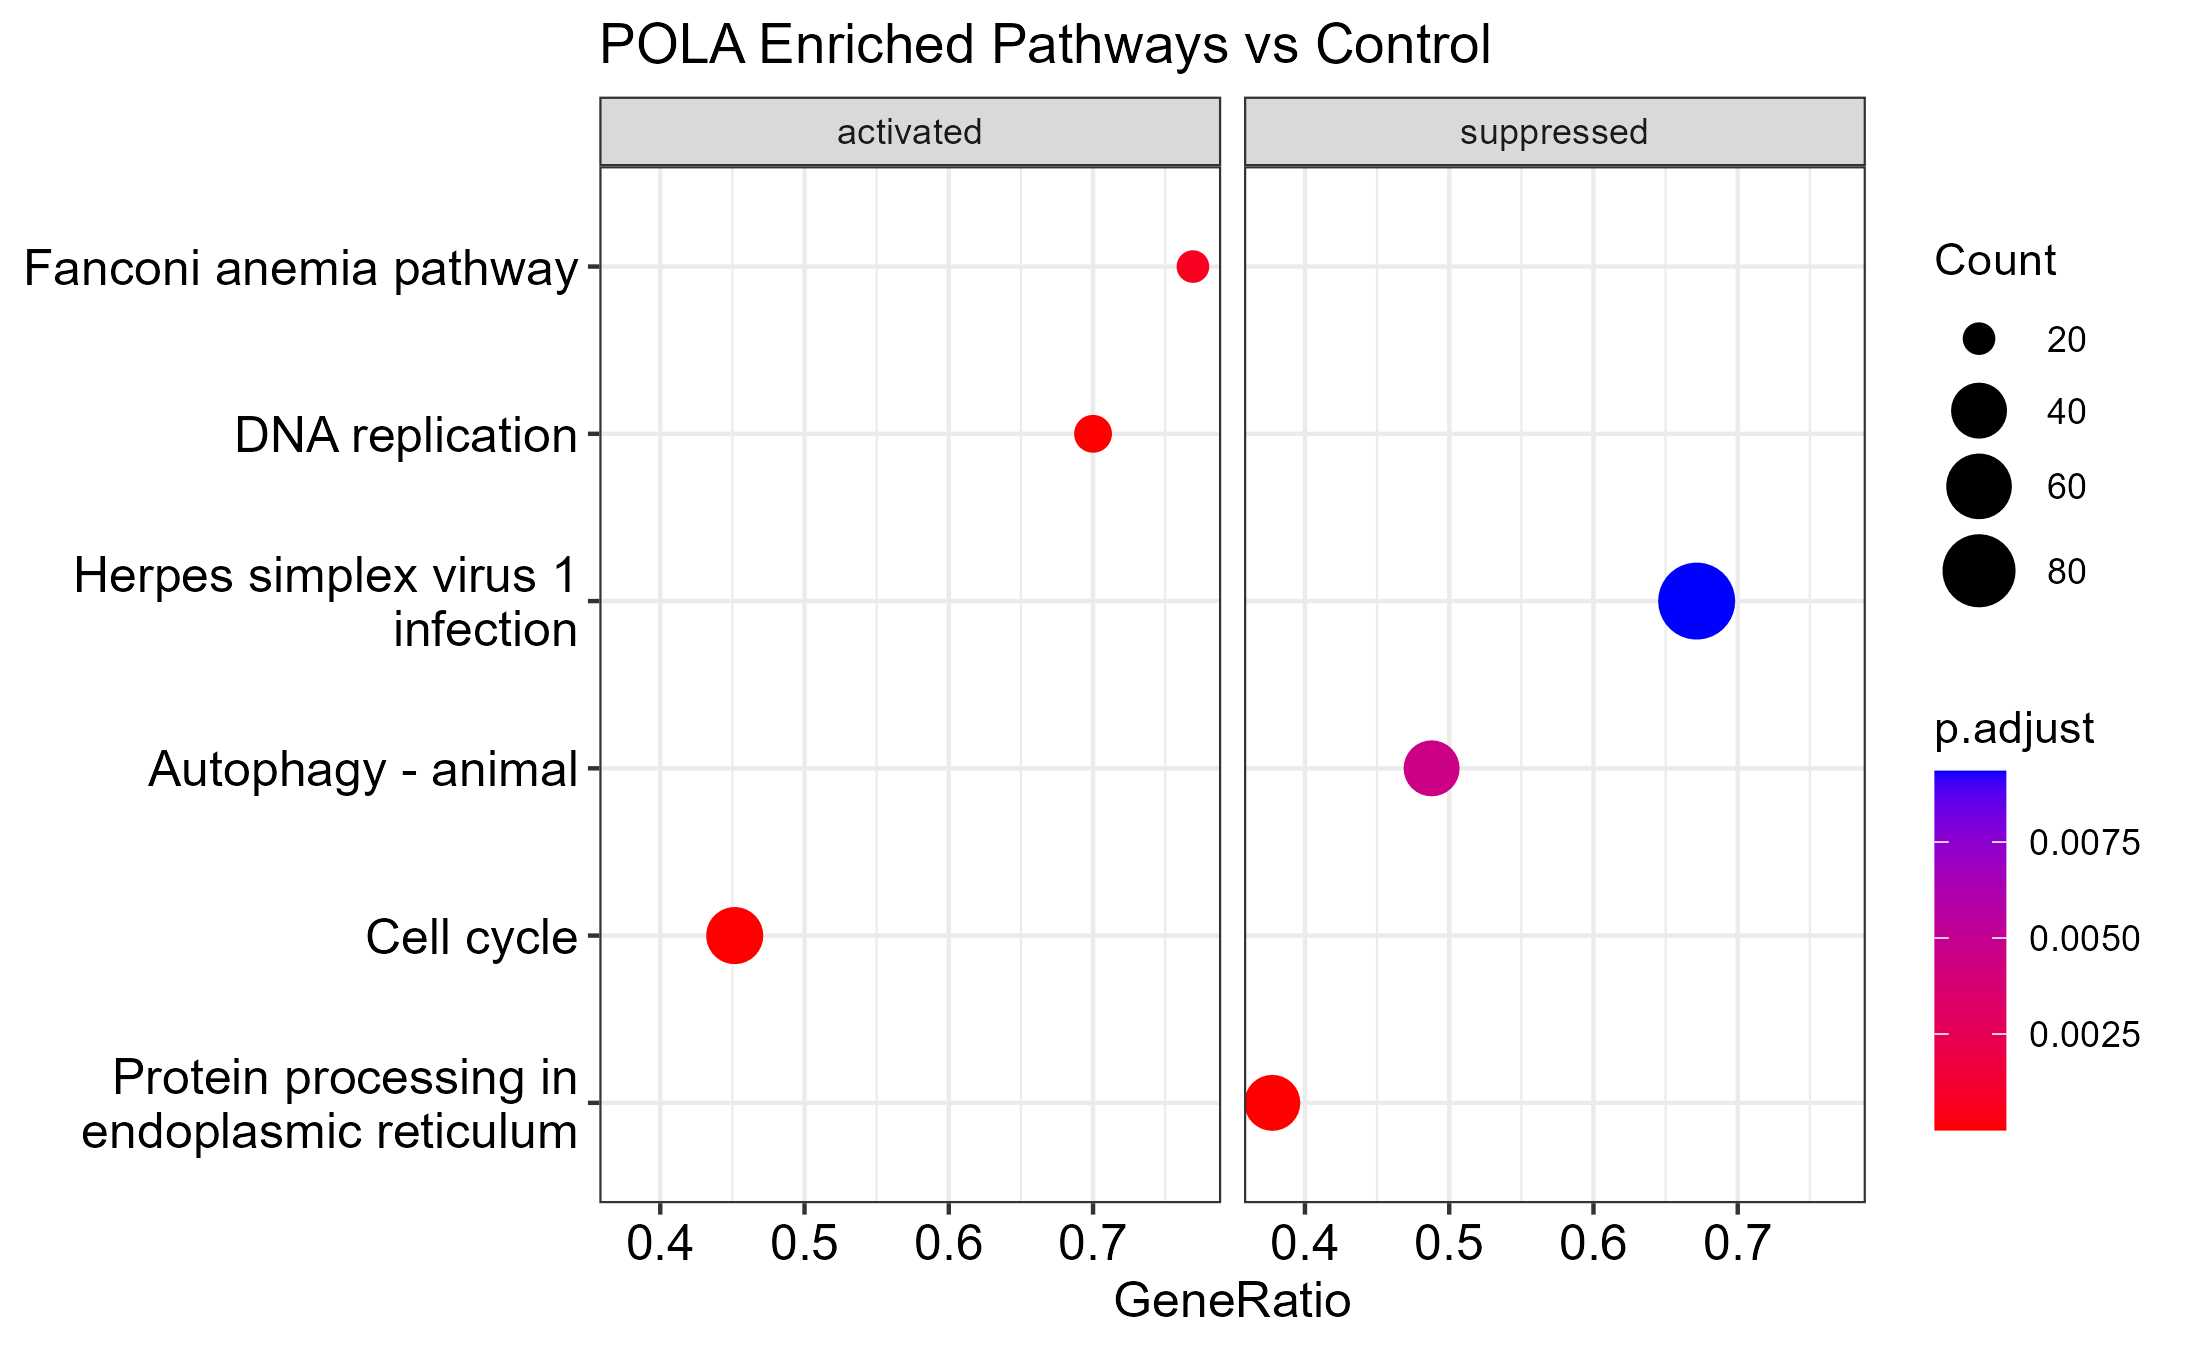
\includegraphics[width=0.49\textwidth]{figures/ch3-Model Development/POLA GSEA.png}};
\end{figure} 

\begin{figure}[h!]
  \centering
  {\phantomsubcaption\label{fig:OPLA NASH}}
  {\phantomsubcaption\label{fig:POLA NASH}}
  \tikz\node[inner sep=0pt,label={[anchor=north west]north west:\subref{fig:OPLA NASH}}] {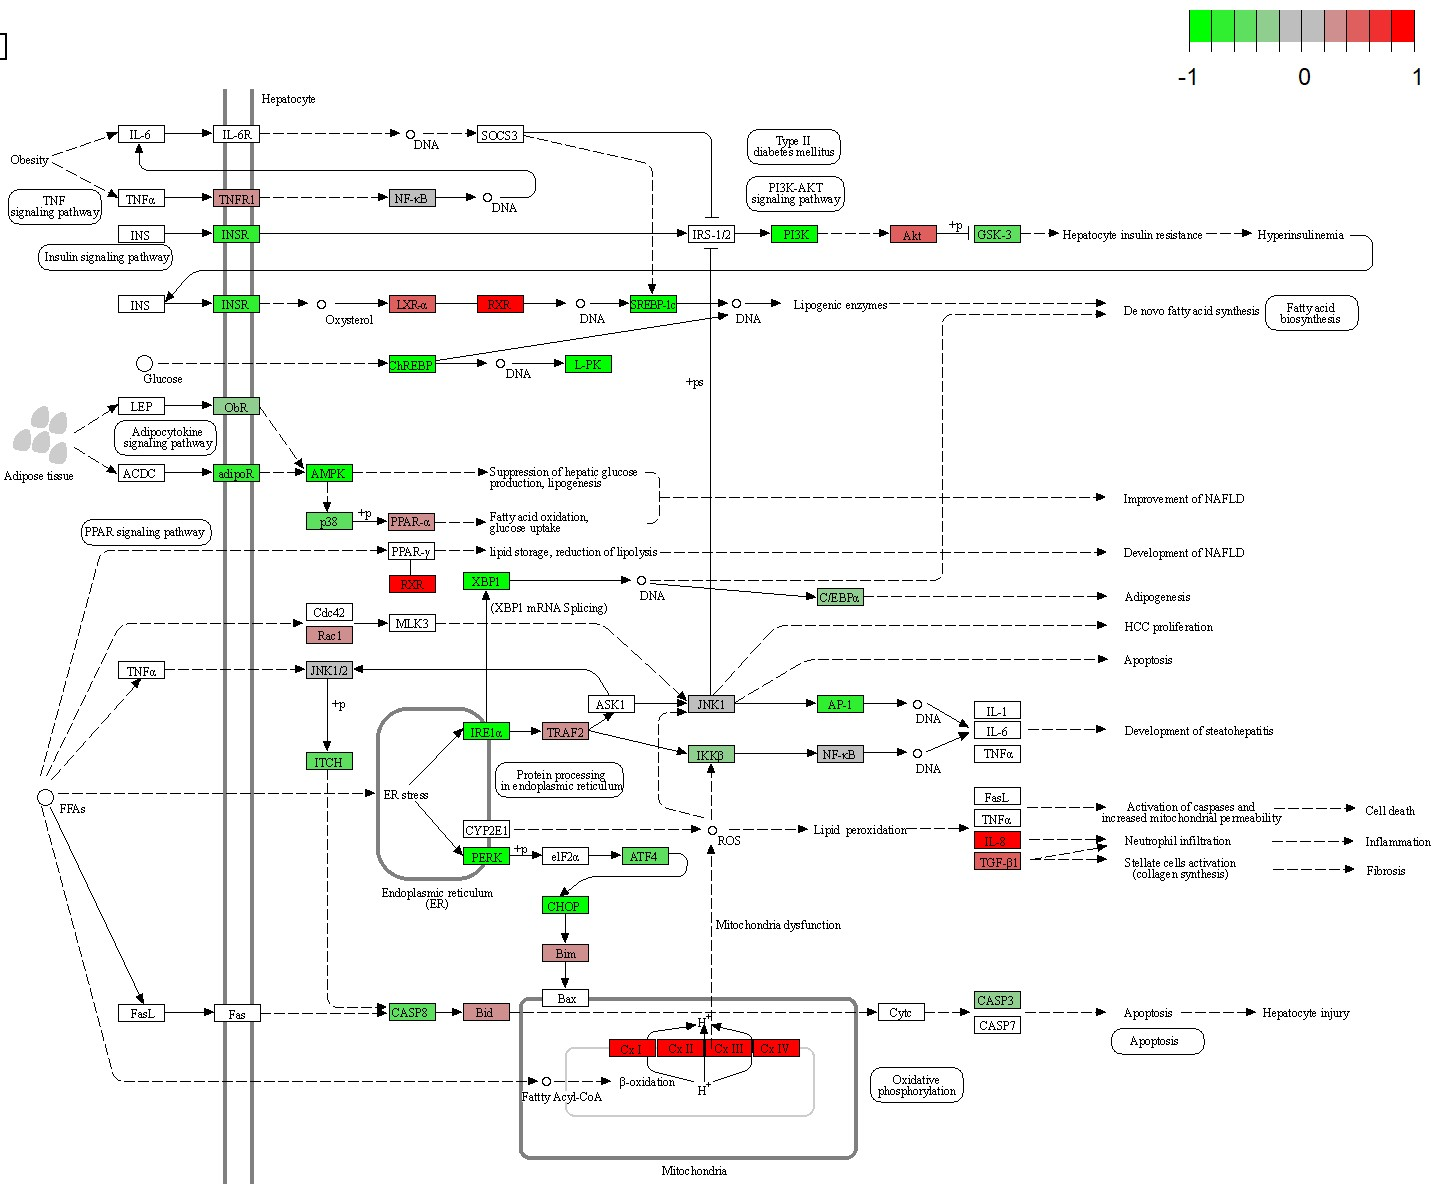
\includegraphics[width=0.49\textwidth]{figures/ch3-Model Development/OPLA NASH.jpg}};
  \tikz\node[inner sep=0pt,label={[anchor=north west]north west:\subref{fig:POLA NASH}}] {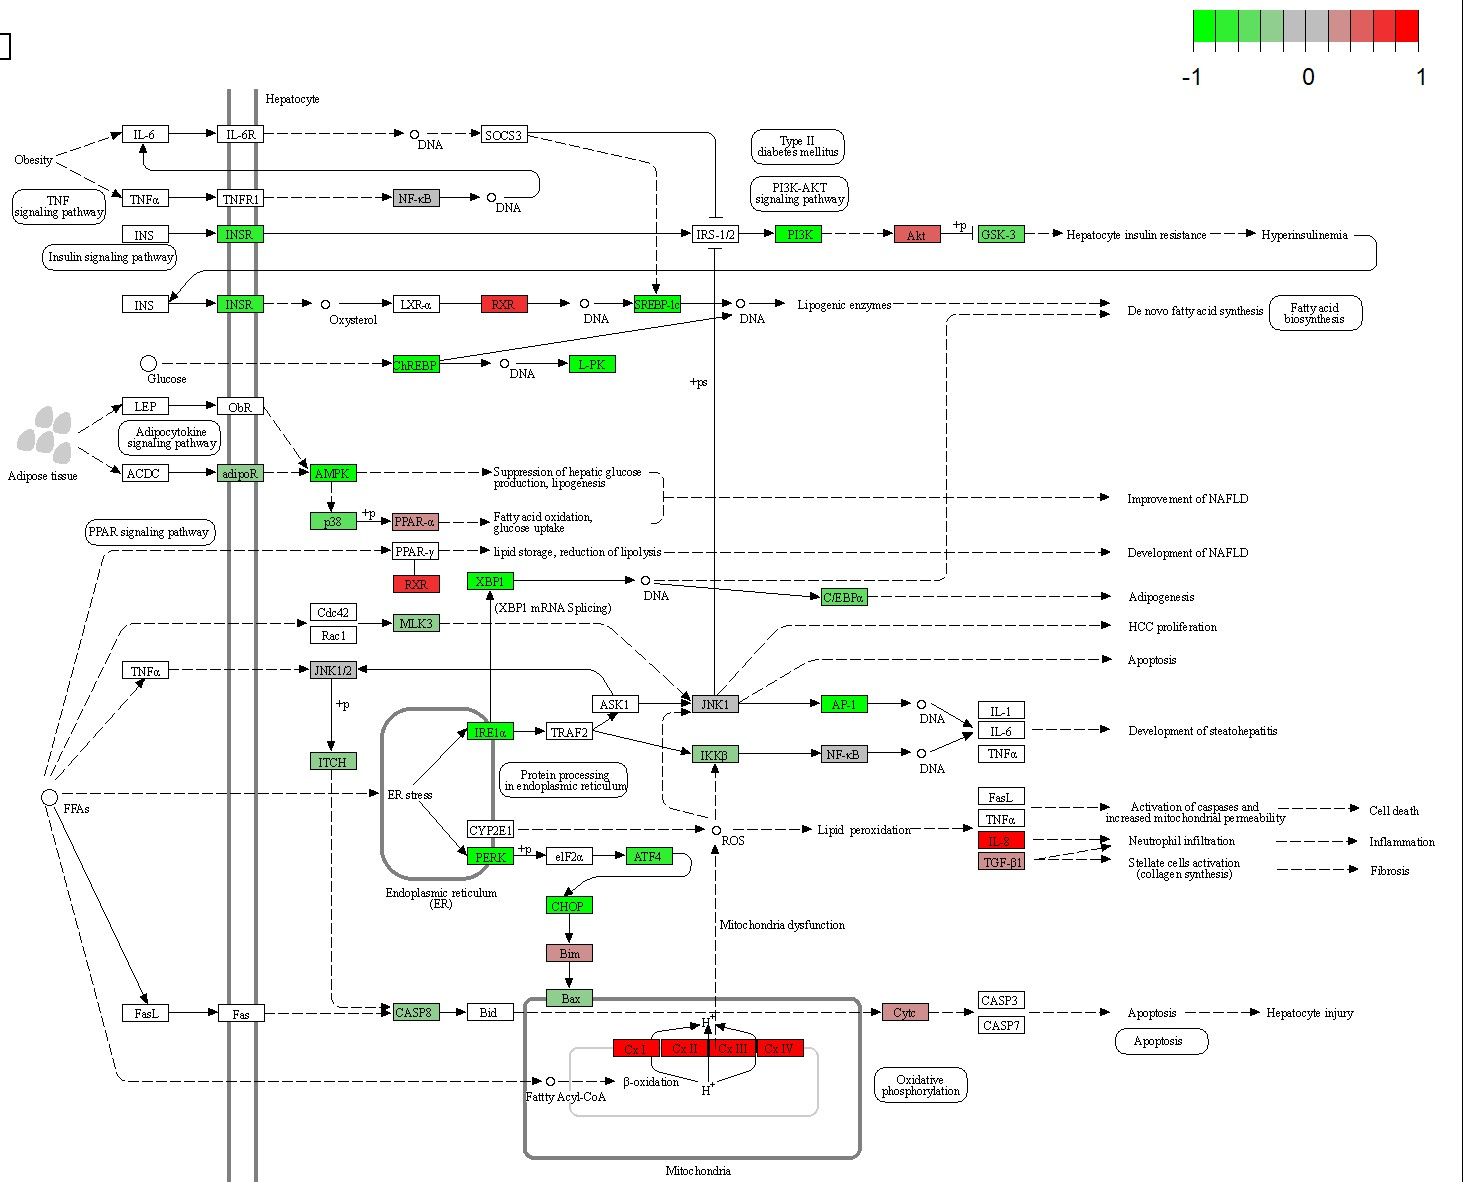
\includegraphics[width=0.49\textwidth]{figures/ch3-Model Development/POLA NASH.jpg}};
\end{figure}